% Signal at pin 2 as a function of the CPU clock cycles
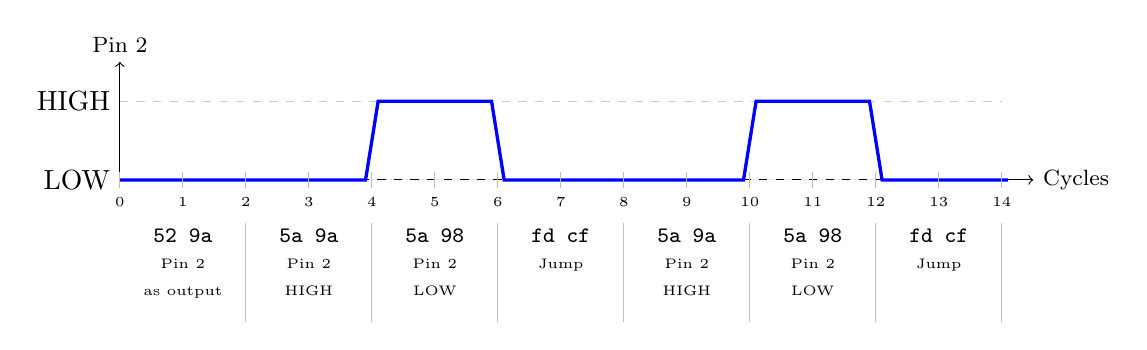
\begin{tikzpicture}[x=0.8cm, y=1cm]
\draw[->] (0,0) -- (14.5,0) node[right] {\footnotesize Cycles};
\draw[->] (0,-0.1) -- (0,1.5) node[above] {\footnotesize Pin 2};
\draw (0,0) node[left]{LOW};
\draw (0,1) node[left]{HIGH};
\draw[dashed, gray!40] (0,1) -- (14,1);
\draw[dashed, gray!20] (0,0) -- (14,0);
\draw[very thick, blue]
    (0,0) -- (3.9,0) -- (4.1,1) -- (5.9,1) -- (6.1,0) -- (9.9,0)
    -- (10.1,1) -- (11.9,1) -- (12.1,0) -- (14.1,0);
\foreach \x in {0,...,14} {
    \draw[gray!50] (\x, -0.1) -- (\x, 0.1);
    \node[below] at (\x, -0.1) {\tiny \x};
}
\foreach \a/\b/\t in {0/2/{\texttt{52 9a}\\\tiny Pin 2\\\tiny as output},
                      2/4/{\texttt{5a 9a}\\\tiny Pin 2\\\tiny HIGH},
                      4/6/{\texttt{5a 98}\\\tiny Pin 2\\\tiny LOW},
                      6/8/{\texttt{fd cf}\\\tiny Jump},
                      8/10/{\texttt{5a 9a}\\\tiny Pin 2\\\tiny HIGH},
                      10/12/{\texttt{5a 98}\\\tiny Pin 2\\\tiny LOW},
                      12/14/{\texttt{fd cf}\\\tiny Jump}} {
    \node[font=\footnotesize, align=center, anchor=north] at ({(\a+\b)/2}, -0.5) {\t};
    \draw[gray!50] (\b, -0.55) -- (\b, -1.8);
}
\end{tikzpicture}
